\documentclass{extbook}[14pt]
\usepackage{multicol, enumerate, enumitem, hyperref, color, soul, setspace, parskip, fancyhdr, amssymb, amsthm, amsmath, bbm, latexsym, units, mathtools}
\everymath{\displaystyle}
\usepackage[headsep=0.5cm,headheight=0cm, left=1 in,right= 1 in,top= 1 in,bottom= 1 in]{geometry}
\usepackage{dashrule}  % Package to use the command below to create lines between items
\newcommand{\litem}[1]{\item #1

\rule{\textwidth}{0.4pt}}
\pagestyle{fancy}
\lhead{}
\chead{Answer Key for Makeup Progress Quiz -1 Version A}
\rhead{}
\lfoot{7547-2949}
\cfoot{}
\rfoot{Fall 2020}
\begin{document}
\textbf{This key should allow you to understand why you choose the option you did (beyond just getting a question right or wrong). \href{https://xronos.clas.ufl.edu/mac1105spring2020/courseDescriptionAndMisc/Exams/LearningFromResults}{More instructions on how to use this key can be found here}.}

\textbf{If you have a suggestion to make the keys better, \href{https://forms.gle/CZkbZmPbC9XALEE88}{please fill out the short survey here}.}

\textit{Note: This key is auto-generated and may contain issues and/or errors. The keys are reviewed after each exam to ensure grading is done accurately. If there are issues (like duplicate options), they are noted in the offline gradebook. The keys are a work-in-progress to give students as many resources to improve as possible.}

\rule{\textwidth}{0.4pt}

\begin{enumerate}\litem{
Describe the end behavior of the polynomial below.
\[ f(x) = -9(x + 8)^{3}(x - 8)^{8}(x + 7)^{5}(x - 7)^{6} \]

The solution is the graph below, which is option B.
\begin{center}
    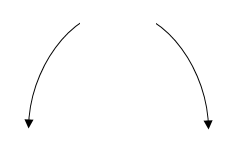
\includegraphics[width=0.3\textwidth]{../Figures/polyEndBehaviorBA.png}
\end{center}\begin{enumerate}[label=\Alph*.]
\begin{multicols}{2}
\item 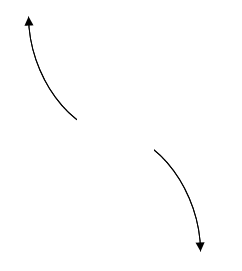
\includegraphics[width = 0.3\textwidth]{../Figures/polyEndBehaviorAA.png}
\item 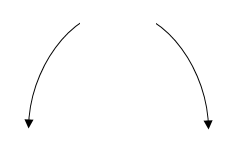
\includegraphics[width = 0.3\textwidth]{../Figures/polyEndBehaviorBA.png}
\item 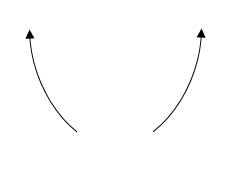
\includegraphics[width = 0.3\textwidth]{../Figures/polyEndBehaviorCA.png}
\item 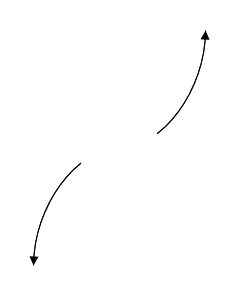
\includegraphics[width = 0.3\textwidth]{../Figures/polyEndBehaviorDA.png}
\end{multicols}\item None of the above.\end{enumerate}
\textbf{General Comment:} Remember that end behavior is determined by the leading coefficient AND whether the \textbf{sum} of the multiplicities is positive or negative.
}
\litem{
Describe the zero behavior of the zero $x = 2$ of the polynomial below.
\[ f(x) = 2(x + 4)^{7}(x - 4)^{6}(x - 2)^{10}(x + 2)^{7} \]

The solution is the graph below, which is option C.
\begin{center}
    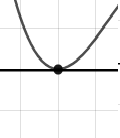
\includegraphics[width=0.3\textwidth]{../Figures/polyZeroBehaviorCopyCA.png}
\end{center}\begin{enumerate}[label=\Alph*.]
\begin{multicols}{2}
\item 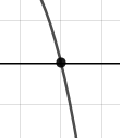
\includegraphics[width = 0.3\textwidth]{../Figures/polyZeroBehaviorCopyAA.png}
\item 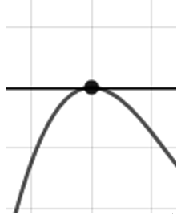
\includegraphics[width = 0.3\textwidth]{../Figures/polyZeroBehaviorCopyBA.png}
\item 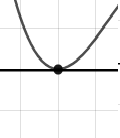
\includegraphics[width = 0.3\textwidth]{../Figures/polyZeroBehaviorCopyCA.png}
\item 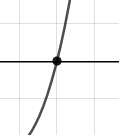
\includegraphics[width = 0.3\textwidth]{../Figures/polyZeroBehaviorCopyDA.png}
\end{multicols}\item None of the above.\end{enumerate}
\textbf{General Comment:} You will need to sketch the entire graph, then zoom in on the zero the question asks about.
}
\litem{
Construct the lowest-degree polynomial given the zeros below. Then, choose the intervals that contain the coefficients of the polynomial in the form $x^3+bx^2+cx+d$.
\[ -5 + 3 i \text{ and } -1 \]

The solution is \( x^{3} +11 x^{2} +44 x + 34 \), which is option B.\begin{enumerate}[label=\Alph*.]
\item \( b \in [-3, 5], c \in [5, 16], \text{ and } d \in [-2, 9] \)

$x^{3} + x^{2} +6 x + 5$, which corresponds to multiplying out $(x + 5)(x + 1)$.
\item \( b \in [10, 15], c \in [39, 51], \text{ and } d \in [33, 40] \)

* $x^{3} +11 x^{2} +44 x + 34$, which is the correct option.
\item \( b \in [-3, 5], c \in [-2, 1], \text{ and } d \in [-11, -2] \)

$x^{3} + x^{2} -2 x -3$, which corresponds to multiplying out $(x -3)(x + 1)$.
\item \( b \in [-16, -7], c \in [39, 51], \text{ and } d \in [-42, -25] \)

$x^{3} -11 x^{2} +44 x -34$, which corresponds to multiplying out $(x-(-5 + 3 i))(x-(-5 - 3 i))(x -1)$.
\item \( \text{None of the above.} \)

This corresponds to making an unanticipated error or not understanding how to use nonreal complex numbers to create the lowest-degree polynomial. If you chose this and are not sure what you did wrong, please contact the coordinator for help.
\end{enumerate}

\textbf{General Comment:} Remember that the conjugate of $a+bi$ is $a-bi$. Since these zeros always come in pairs, we need to multiply out $(x-(-5 + 3 i))(x-(-5 - 3 i))(x-(-1))$.
}
\litem{
Describe the zero behavior of the zero $x = 8$ of the polynomial below.
\[ f(x) = 6(x + 2)^{9}(x - 2)^{8}(x + 8)^{7}(x - 8)^{4} \]

The solution is the graph below, which is option C.
\begin{center}
    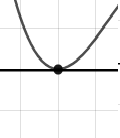
\includegraphics[width=0.3\textwidth]{../Figures/polyZeroBehaviorCA.png}
\end{center}\begin{enumerate}[label=\Alph*.]
\begin{multicols}{2}
\item 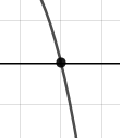
\includegraphics[width = 0.3\textwidth]{../Figures/polyZeroBehaviorAA.png}
\item 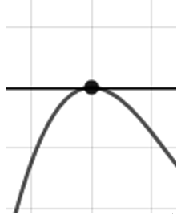
\includegraphics[width = 0.3\textwidth]{../Figures/polyZeroBehaviorBA.png}
\item 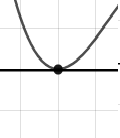
\includegraphics[width = 0.3\textwidth]{../Figures/polyZeroBehaviorCA.png}
\item 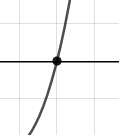
\includegraphics[width = 0.3\textwidth]{../Figures/polyZeroBehaviorDA.png}
\end{multicols}\item None of the above.\end{enumerate}
\textbf{General Comment:} You will need to sketch the entire graph, then zoom in on the zero the question asks about.
}
\litem{
Which of the following equations \textit{could} be of the graph presented below?

\begin{center}
    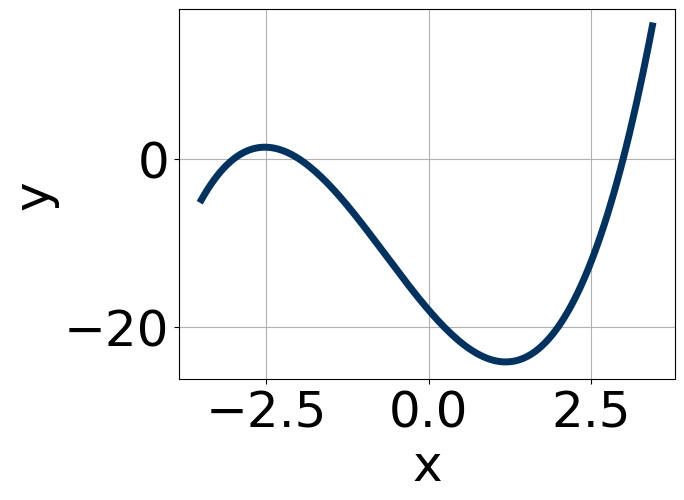
\includegraphics[width=0.5\textwidth]{../Figures/polyGraphToFunctionCopyA.png}
\end{center}




The solution is \( 13(x - 3)^{11} (x + 3)^{9} (x + 2)^{5} \), which is option E.\begin{enumerate}[label=\Alph*.]
\item \( -20(x - 3)^{11} (x + 3)^{7} (x + 2)^{7} \)

This corresponds to the leading coefficient being the opposite value than it should be.
\item \( 15(x - 3)^{4} (x + 3)^{11} (x + 2)^{7} \)

The factor $3$ should have been an odd power.
\item \( -4(x - 3)^{4} (x + 3)^{5} (x + 2)^{9} \)

The factor $(x - 3)$ should have an odd power and the leading coefficient should be the opposite sign.
\item \( 19(x - 3)^{10} (x + 3)^{8} (x + 2)^{5} \)

The factors $3$ and $-3$ have have been odd power.
\item \( 13(x - 3)^{11} (x + 3)^{9} (x + 2)^{5} \)

* This is the correct option.
\end{enumerate}

\textbf{General Comment:} General Comments: Draw the x-axis to determine which zeros are touching (and so have even multiplicity) or cross (and have odd multiplicity).
}
\litem{
Which of the following equations \textit{could} be of the graph presented below?

\begin{center}
    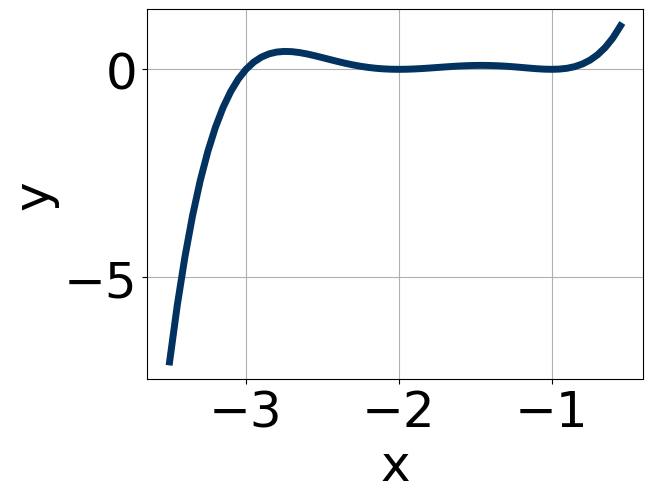
\includegraphics[width=0.5\textwidth]{../Figures/polyGraphToFunctionA.png}
\end{center}




The solution is \( 16(x + 1)^{10} (x + 2)^{8} (x + 3)^{9} \), which is option A.\begin{enumerate}[label=\Alph*.]
\item \( 16(x + 1)^{10} (x + 2)^{8} (x + 3)^{9} \)

* This is the correct option.
\item \( 11(x + 1)^{4} (x + 2)^{11} (x + 3)^{7} \)

The factor $(x + 2)$ should have an even power.
\item \( -3(x + 1)^{10} (x + 2)^{4} (x + 3)^{4} \)

The factor $(x + 3)$ should have an odd power and the leading coefficient should be the opposite sign.
\item \( -16(x + 1)^{6} (x + 2)^{6} (x + 3)^{11} \)

This corresponds to the leading coefficient being the opposite value than it should be.
\item \( 12(x + 1)^{8} (x + 2)^{11} (x + 3)^{4} \)

The factor $(x + 2)$ should have an even power and the factor $(x + 3)$ should have an odd power.
\end{enumerate}

\textbf{General Comment:} General Comments: Draw the x-axis to determine which zeros are touching (and so have even multiplicity) or cross (and have odd multiplicity).
}
\litem{
Describe the end behavior of the polynomial below.
\[ f(x) = 9(x + 4)^{2}(x - 4)^{5}(x + 8)^{3}(x - 8)^{4} \]

The solution is the graph below, which is option C.
\begin{center}
    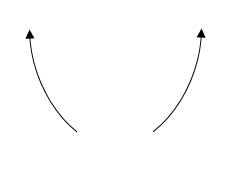
\includegraphics[width=0.3\textwidth]{../Figures/polyEndBehaviorCopyCA.png}
\end{center}\begin{enumerate}[label=\Alph*.]
\begin{multicols}{2}
\item 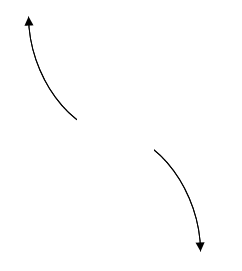
\includegraphics[width = 0.3\textwidth]{../Figures/polyEndBehaviorCopyAA.png}
\item 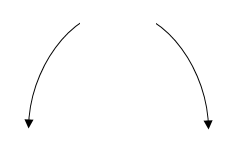
\includegraphics[width = 0.3\textwidth]{../Figures/polyEndBehaviorCopyBA.png}
\item 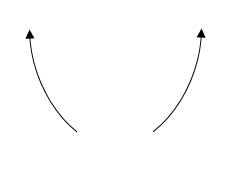
\includegraphics[width = 0.3\textwidth]{../Figures/polyEndBehaviorCopyCA.png}
\item 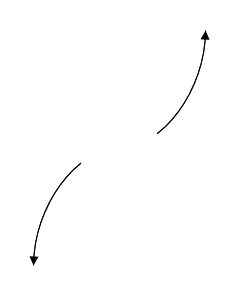
\includegraphics[width = 0.3\textwidth]{../Figures/polyEndBehaviorCopyDA.png}
\end{multicols}\item None of the above.\end{enumerate}
\textbf{General Comment:} Remember that end behavior is determined by the leading coefficient AND whether the \textbf{sum} of the multiplicities is positive or negative.
}
\litem{
Construct the lowest-degree polynomial given the zeros below. Then, choose the intervals that contain the coefficients of the polynomial in the form $ax^3+bx^2+cx+d$.
\[ \frac{1}{2}, -5, \text{ and } \frac{-3}{4} \]

The solution is \( 8x^{3} +42 x^{2} +7 x -15 \), which is option D.\begin{enumerate}[label=\Alph*.]
\item \( a \in [1, 9], b \in [50, 52], c \in [46, 55], \text{ and } d \in [12, 18] \)

$8x^{3} +50 x^{2} +53 x + 15$, which corresponds to multiplying out $(2x + 1)(x + 5)(4x + 3)$.
\item \( a \in [1, 9], b \in [35, 44], c \in [6, 12], \text{ and } d \in [12, 18] \)

$8x^{3} +42 x^{2} +7 x + 15$, which corresponds to multiplying everything correctly except the constant term.
\item \( a \in [1, 9], b \in [-32, -28], c \in [-48, -38], \text{ and } d \in [-16, -13] \)

$8x^{3} -30 x^{2} -47 x -15$, which corresponds to multiplying out $(2x + 1)(x -5)(4x + 3)$.
\item \( a \in [1, 9], b \in [35, 44], c \in [6, 12], \text{ and } d \in [-16, -13] \)

* $8x^{3} +42 x^{2} +7 x -15$, which is the correct option.
\item \( a \in [1, 9], b \in [-50, -37], c \in [6, 12], \text{ and } d \in [12, 18] \)

$8x^{3} -42 x^{2} +7 x + 15$, which corresponds to multiplying out $(2x + 1)(x -5)(4x -3)$.
\end{enumerate}

\textbf{General Comment:} To construct the lowest-degree polynomial, you want to multiply out $(2x -1)(x + 5)(4x + 3)$
}
\litem{
Construct the lowest-degree polynomial given the zeros below. Then, choose the intervals that contain the coefficients of the polynomial in the form $x^3+bx^2+cx+d$.
\[ 3 - 3 i \text{ and } 4 \]

The solution is \( x^{3} -10 x^{2} +42 x -72 \), which is option B.\begin{enumerate}[label=\Alph*.]
\item \( b \in [8, 14], c \in [39, 42.7], \text{ and } d \in [66, 81] \)

$x^{3} +10 x^{2} +42 x + 72$, which corresponds to multiplying out $(x-(3 - 3 i))(x-(3 + 3 i))(x + 4)$.
\item \( b \in [-11, -7], c \in [39, 42.7], \text{ and } d \in [-75, -67] \)

* $x^{3} -10 x^{2} +42 x -72$, which is the correct option.
\item \( b \in [-8, 2], c \in [-7.7, -5.8], \text{ and } d \in [12, 17] \)

$x^{3} + x^{2} -7 x + 12$, which corresponds to multiplying out $(x -3)(x -4)$.
\item \( b \in [-8, 2], c \in [-2.9, 0.2], \text{ and } d \in [-19, -11] \)

$x^{3} + x^{2} -x -12$, which corresponds to multiplying out $(x + 3)(x -4)$.
\item \( \text{None of the above.} \)

This corresponds to making an unanticipated error or not understanding how to use nonreal complex numbers to create the lowest-degree polynomial. If you chose this and are not sure what you did wrong, please contact the coordinator for help.
\end{enumerate}

\textbf{General Comment:} Remember that the conjugate of $a+bi$ is $a-bi$. Since these zeros always come in pairs, we need to multiply out $(x-(3 - 3 i))(x-(3 + 3 i))(x-(4))$.
}
\litem{
Construct the lowest-degree polynomial given the zeros below. Then, choose the intervals that contain the coefficients of the polynomial in the form $ax^3+bx^2+cx+d$.
\[ 5, \frac{6}{5}, \text{ and } 1 \]

The solution is \( 5x^{3} -36 x^{2} +61 x -30 \), which is option A.\begin{enumerate}[label=\Alph*.]
\item \( a \in [-2, 6], b \in [-37, -32], c \in [56, 63], \text{ and } d \in [-34, -28] \)

* $5x^{3} -36 x^{2} +61 x -30$, which is the correct option.
\item \( a \in [-2, 6], b \in [-37, -32], c \in [56, 63], \text{ and } d \in [29, 33] \)

$5x^{3} -36 x^{2} +61 x + 30$, which corresponds to multiplying everything correctly except the constant term.
\item \( a \in [-2, 6], b \in [8, 19], c \in [-51, -45], \text{ and } d \in [29, 33] \)

$5x^{3} +14 x^{2} -49 x + 30$, which corresponds to multiplying out $(x + 5)(5x -6)(x -1)$.
\item \( a \in [-2, 6], b \in [35, 40], c \in [56, 63], \text{ and } d \in [29, 33] \)

$5x^{3} +36 x^{2} +61 x + 30$, which corresponds to multiplying out $(x + 5)(5x + 6)(x + 1)$.
\item \( a \in [-2, 6], b \in [22, 27], c \in [-9, 0], \text{ and } d \in [-34, -28] \)

$5x^{3} +26 x^{2} -x -30$, which corresponds to multiplying out $(x + 5)(5x + 6)(x -1)$.
\end{enumerate}

\textbf{General Comment:} To construct the lowest-degree polynomial, you want to multiply out $(x -5)(5x -6)(x -1)$
}
\end{enumerate}

\end{document}